\documentclass[a4paper]{article}
\usepackage[UTF8]{ctex}
\usepackage{geometry}
\usepackage{graphicx}
\usepackage{url}
\usepackage{multirow}
\usepackage{array}
\usepackage{booktabs}
\usepackage{url}
\usepackage{enumitem}
\usepackage{graphicx}
\usepackage{float}
\usepackage{amssymb}
\usepackage{amsmath}
\usepackage{subfig}
\usepackage{longtable}

\geometry{a4paper, scale=0.78}

\title{Math Basis 04}
\author{Chen Gong}
\date{21 October 2019}

\begin{document}

\maketitle
本节主要的内容是描述琴生不等式(Jensen's Inequality)。有关琴生不等式的描述为,如果函数$f(x)$为凸函数(convex function),那么有$\mathbb{E}[f(x)]\geq f(\mathbb{E}[x])$。

\section{Jensen's Inequality中的证明}
\begin{figure}[H]
    \centering
    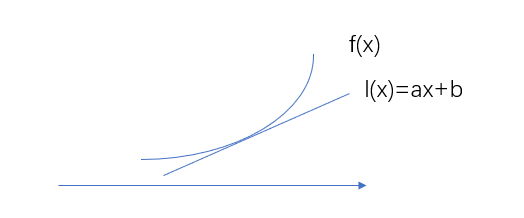
\includegraphics[width=.5\textwidth]{微信图片_20191021084621.png}
    \caption{函数和它在某点的切线的表达式}
    \label{fig:my_label_1}
\end{figure}

设切点的横坐标为$\mathbb{E}[x]$,那么$f(\mathbb{E}[x])=L(x)=a\mathbb{E}[x]+b$。又因为function为convex function。那么很显然,对于$\forall x$都有$f(x)\geq L(x)$。然后,我们同时对不等式两边求期望,可以得到$\mathbb{E}[f(x)]\geq \mathbb{E}[L(x)]$。那么我们进行如下的推导:
\begin{equation}
    \begin{split}
        \mathbb{E}[f(x)]\geq & \mathbb{E}[L(x)] \\
        = & \mathbb{E}[a\mathbb{E}[x]+b] \\
        = & a\mathbb{E}[x] + b \\
        = & f(\mathbb{E}[x]) \\
    \end{split}
\end{equation}
可以很简单的得出结论。

\section{Jensen's Inequality的推广}
假设$c$是$[a,b]$之间的任意一点,我们可以很自然的描述为$c=ta+(1-t)b$。我们可以使用Jensen's Inequality的推广形式。这个不等式的证明很简单,结论也很直觉性(肯定是这样的),此处不再做更多的描述。Jensen's Inequality将在后续相关的知识中大量的使用,故此处暂做补充。
\begin{equation}
    tf(a)+(1-t)f(b)\geq f(ta+(1-t)b)
\end{equation}

\end{document}
